\documentclass[11pt,a4paper]{article}
\usepackage[T1]{fontenc}
\usepackage[utf8]{inputenc}
\usepackage[british]{babel}
\usepackage{lmodern,microtype}
\usepackage{csquotes}
\usepackage[a4paper,margin=28mm]{geometry}
\setlength{\emergencystretch}{2em}
\usepackage{amsmath,amssymb,amsthm,mathtools,bm}
\usepackage{booktabs,longtable,tabularx,array}
\usepackage{enumitem}
\usepackage{xcolor}
\usepackage{tikz}
\usetikzlibrary{arrows.meta,calc,fit,positioning,shapes.geometric,backgrounds}
\usepackage{graphicx}
\graphicspath{{../../FIGURES/EXPORT/}}
\usepackage[colorlinks=true,allcolors=blue!55!black]{hyperref}
\usepackage[nameinlink,noabbrev]{cleveref}
\usepackage[backend=biber,style=authoryear,sorting=nyt,sortcites=true,
  maxcitenames=3,giveninits=true,uniquename=init,dashed=false,
  useprefix=true,doi=true,isbn=false,url=true]{biblatex}
\addbibresource{references.bib}
\DeclareDelimFormat{nameyeardelim}{\addcomma\space}

\newtheorem{theorem}{Theorem}[section]
\newtheorem{proposition}[theorem]{Proposition}
\newtheorem{lemma}[theorem]{Lemma}
\newtheorem{corollary}[theorem]{Corollary}
\newtheorem{definition}[theorem]{Definition}
\newtheorem{remark}[theorem]{Remark}
\newtheorem{counterexample}[theorem]{Counterexample}
\newcommand{\C}{\mathbb C}
\newcommand{\R}{\mathbb R}
\newcommand{\Q}{\mathbb Q}
\newcommand{\N}{\mathbb N}
\newcommand{\e}{\varepsilon}
\newcommand{\ord}{\operatorname{ord}}
\newcommand{\inw}{\operatorname{in}}
\newcommand{\supp}{\operatorname{supp}}
\newcommand{\conv}{\operatorname{conv}}
\newcommand{\diag}{\operatorname{diag}}
\newcommand{\Proj}{\operatorname{Proj}}
\newcommand{\Span}{\operatorname{span}}
\newcommand{\closure}{\overline}
\newcommand{\evidence}[1]{\textsf{#1}}
\newcommand{\paperone}{Paper~I}

\title{Kernel-Checked Opening Theory and Coefficient-Sensitive Newton Geometry\\
of a Six-State Dark Quantum Channel}
\author{Zach Medford\\[-1mm]\small Independent research preprint}
\date{Version R2.1 --- 10 August 2026\\
\small\href{https://github.com/SLresearch74/Signed-Involution-Sector-Exclusion-for-EZT-in-Finite-Magnetic-Graph-Hamiltonians---v1.0.0}{Repository and reproducibility materials}}

\begin{document}
\maketitle
\begin{abstract}
Exact zero transfer in a finite quantum channel is a statement about every
time, whereas the loss of one symmetry certificate concerns only one proof.
This paper gives a kernel-checked local opening theory for a locked six-state
real Hamiltonian under internal diagonal perturbations.  In Lean~4 with
Mathlib, we formalise the signed involutions and all-depth baseline darkness,
the unreduced selected cofactor, the pointwise dark-plane decomposition,
endpoint word support, the complete fixed-ray trichotomy, the fixed-fibre
Newton theorem and the analytic bridge to the actual matrix exponential.  The
selected resolvent numerator is
\(
L(z^2+2z)+2Q(z+1)+R
\), where
\(L=d_1-d_2+d_3-d_4\), \(Q=d_2d_4-d_1d_3\), and
\(R=d_1d_2(d_3-d_4)+d_3d_4(d_1-d_2)\).
The formal development proves that the two fixed non-dark fibres have Newton
polyhedra \((1,3)+\R_{\ge0}^2\) and \((2,4)+\R_{\ge0}^2\), while the dark fibre
is empty, and identifies these coefficients with the convergent amplitude
series.  Beyond that verified spine, conventional exact proofs establish
monomial-fibre aggregation, a moving-arc lower-hull classification, a
four-vertex universal Newton polyhedron, a 16-cone Gr\"obner fan and a
fixed-weight Noetherian termination theorem.  The paper marks this verification
boundary explicitly: no effective uniform depth bound, finite global recursive
atlas, or blanket formalisation claim is made.

\end{abstract}
\noindent\textbf{Evidence convention.}
Claims carrying an explicit status use only \evidence{PROVED},
\evidence{KERNEL-CHECKED}, \evidence{VERIFIED-EXACT},
\evidence{VERIFIED-BYTE}, \evidence{MEASURED} with a sample size,
\evidence{FALSIFIED}, \evidence{CONJECTURE}, or \evidence{UNAVAILABLE}.
\evidence{KERNEL-CHECKED} means that the stated Lean theorem and its
dependencies were accepted by the pinned Lean kernel; it does not extend to
nearby results not named in the traceability map.  A computed identity is never
promoted to a theorem without a proof, and a failed certificate is never called
an opening.

\tableofcontents

\section{Introduction}\label{sec:introduction}

Dark states and destructive interference are standard mechanisms in coherent
population trapping and adiabatic transfer \parencite{Aspect1988,Gaubatz1990}.
Recent work gives broad structural descriptions of dark states in multilevel
systems \parencite{Zhao2026}; continuous-time quantum-walk research likewise
studies exact or near suppression of transfer \parencite{Sett2019,Godsil2012},
while time-reversal breaking is known to alter quantum transport
\parencite{Zimboras2013}.  Those settings motivate, but do not answer, the
local algebraic question studied here: once a channel is exactly dark, which
coefficient is the first to survive under a declared diagonal perturbation,
and how does that answer change under multi-scale substitution?

The central contribution is not only an exact answer for one locked channel,
but a machine-checked proof of its fixed-ray and fixed-fibre spine.  The model,
signed-symmetry argument, determinant identity, word recurrence, coefficient
support, branch classification, convex-geometric conclusion and
matrix-exponential bridge have been formalised in Lean~4
\parencite{deMouraUllrich2021} using Mathlib
\parencite{MathlibCommunity2020}.  This changes the evidentiary architecture of
the paper: exact scripts are retained as independent checks, while the main
finite-algebra chain is anchored to named kernel-checked theorems.  The precise
map and trust boundary appear in \cref{sec:formalisation}.

The companion \paperone{} proves that, for a finite Hamiltonian $H$, exact
zero transfer from $e_0$ to $e_5$ is equivalent to the vanishing of all
moments $e_5^{\mathsf T}H^ke_0$, to orthogonality of $e_5$ to the source
Krylov space, and to the corresponding spectral-projector conditions
\parencite{MedfordPaperI}.  Signed involutions provide sufficient exclusion
certificates there.  This paper starts from those equivalences and develops the
coefficient-sensitive geometry of one six-state channel.  It does not repeat
the graph atlas, magnetic-flux examples, norm bounds, mass estimates or
open-system extensions of \paperone.

The first fixed-direction version appeared in the author-supplied R1.2
manuscript \parencite{MedfordR12}.  The present version retains its exact
numerator and trichotomy, supplies the complete Lean formalisation through the
analytic bridge, repairs the scope of moving-direction cancellation, and adds
endpoint words, pullback aggregation, analytic arcs, universal coordinates,
Gr\"obner/Rees data and the fixed-weight Noetherian termination theorem.

\subsection{Contribution and evidence structure}

Resolvents and Markov parameters are standard in realisation and transfer
theory \parencite{HoKalman1966,Noferini2023}; noncommutative word series are
standard in nonlinear systems and weighted automata
\parencite{Fliess1981,Sakarovitch2009,BerstelReutenauer2010}.  Newton
polyhedra, tropical initial forms, Gr\"obner fans, Rees algebras and arc
contact orders also have mature theories
\parencite{Kouchnirenko1976,Varchenko1976,MaclaganSturmfels2015,Fukuda2007,Ein2004}.
The contribution is their exact synthesis for a channel in which moment and
amplitude faces can genuinely disagree.

The \evidence{KERNEL-CHECKED} contribution comprises:
\begin{enumerate}[label=(\roman*)]
\item two explicit signed involutions and all-depth baseline darkness;
\item the exact unreduced three-coefficient numerator and its coefficient
      syzygy;
\item the pointwise union of two dark planes, each with a persistent signed
      certificate;
\item the locked endpoint-access support theorem and signed boundary power sum;
\item the complete linear/quadratic/exact-zero fixed-ray trichotomy;
\item the two fixed-fibre Newton orthants, empty dark fibre and unique
      positive-weight vertices; and
\item the globally convergent identification of the formal coefficient array
      with the selected matrix-exponential amplitude.
\end{enumerate}

The subsequent, conventionally proved extension comprises monomial-fibre
aggregation, the analytic-arc lower hull and field-corrected tie rule, a
universal four-vertex Newton polyhedron with 15 positive normal cells, a
16-cone Gr\"obner fan and the hierarchy from the dark ideal to a marked
amplitude section, and a non-effective finite decision theorem for every fixed
positive rational weight.  These results are supported by exact symbolic and
combinatorial certificates, but are not labelled \evidence{KERNEL-CHECKED}.

\begin{figure}[ht]
\centering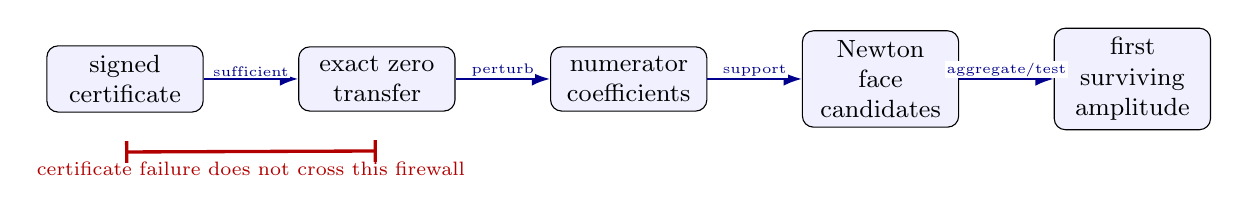
\begin{tikzpicture}[node distance=7mm and 12mm,>=Latex,
  box/.style={draw,rounded corners,fill=blue!6,align=center,minimum height=8mm,text width=17.5mm,font=\small},
  arr/.style={->,thick,blue!55!black}]
\node[box] (cert) {signed\\certificate};
\node[box,right=of cert] (dark) {exact zero\\transfer};
\node[box,right=of dark] (num) {numerator\\coefficients};
\node[box,right=of num] (newt) {Newton face\\candidates};
\node[box,right=of newt] (surv) {first surviving\\amplitude};
\draw[arr] (cert)--node[above,font=\tiny,fill=white,inner sep=.5pt]{sufficient} (dark);
\draw[arr] (dark)--node[above,font=\tiny,fill=white,inner sep=.5pt]{perturb} (num);
\draw[arr] (num)--node[above,font=\tiny,fill=white,inner sep=.5pt]{support} (newt);
\draw[arr] (newt)--node[above,font=\tiny,fill=white,inner sep=.5pt]{aggregate/test} (surv);
\draw[red!70!black,very thick,|-|] ($(cert.south)+(0,-5mm)$)--node[below,font=\scriptsize]{certificate failure does not cross this firewall} ($(dark.south)+(0,-5mm)$);
\end{tikzpicture}

\caption{The logical chain.  The signed-certificate-to-fixed-fibre route and
its amplitude bridge are kernel-checked; later pullback and atlas constructions
extend this core by conventional exact proofs.  Every arrow is one-way unless
an adjacent theorem states an equivalence.}
\label{fig:chain}
\end{figure}

\subsection{Evidence and field conventions}

All algebraic varieties are over a declared field.  The locked physical family
has real diagonal coordinates, while coefficient-torus cancellation is also
studied over \(\C\).  Real non-cancellation conclusions are therefore never
exported to complex leading constants.  Named Lean theorems supply
\evidence{KERNEL-CHECKED} claims; exact computation supplies
\evidence{VERIFIED-EXACT} identities; conventional proofs supply
\evidence{PROVED} claims.  The source census mentioned later is
\evidence{MEASURED} with its sample size.  No numerical sampling establishes a
universal statement.

\paragraph{Scope firewall.}
Closure is not a symmetry certificate; a broken certificate is not an opening;
Newton support is not a surviving coefficient; and the first exponent $p$ of
the perturbation parameter is not the first time power $q$.  Equally, a Lean
proof of the fixed-fibre theorem is not a Lean proof of the later moving-arc or
global-atlas theorems.  These distinctions are maintained throughout.

\section{Formal verification architecture and trust boundary}
\label{sec:formalisation}

The fixed-ray and fixed-fibre core of this paper has been formalised in Lean~4,
an interactive theorem prover with a small proof-checking kernel
\parencite{deMouraUllrich2021}, using the Mathlib library of formalised
mathematics \parencite{MathlibCommunity2020}.  The formalisation is not a
translation of displayed formulas into numerical tests.  It defines the locked
six-state matrix, selected ports, perturbation, cofactor, word coefficients,
coefficient support and real convex hull, and then constructs proof terms for
the corresponding universal statements.

\subsection{End-to-end verified spine}

The organising dependency chain is recorded in \cref{tab:leanmap}.  Module
names and theorem identifiers are part of the release interface: they identify
the exact machine-checked statement rather than a nearby prose summary.

\begin{table}[ht]
\centering
\small
\begin{tabularx}{\textwidth}{@{}p{0.10\textwidth}p{0.34\textwidth}X@{}}
\toprule
Stage & Paper-level claim & Lean module and principal theorem\\
\midrule
M0--M1 & Locked model, signed involutions and all-depth baseline darkness &
\path{M3A.BaselineDarkness}; \path{baseline_moments_dark}\\
M2 & Exact unreduced selected cofactor numerator &
\path{M3A.SelectedNumerator}; \path{selectedNumerator_formula}\\
M3 & Pointwise decomposition into the two dark planes and persistent certificates &
\path{M3A.DarkPlanes}; \path{ell_quad_zero_iff_planes}\\
M4 & Locked endpoint-access support and signed boundary power sum &
\path{M3A.EndpointWords}; \path{sixState_support_bound},
\path{sixState_boundary_ray}\\
M5 & Exact first amplitude coefficients and complete first-order protection on $L=0$ &
\path{M3A.RayCoefficients};
\path{amplitudeCoeff_one_eq_zero_of_linear_zero}\\
M6 & Exhaustive linear/quadratic/dark fixed-ray classification &
\path{M3A.FixedRayTrichotomy}; \path{fixedRay_trichotomy},
\path{classifyRay_spec}\\
M7 & Actual-support Newton orthants and unique positive-weight vertices &
\path{M3A.FixedFibreNewton}; \path{fixedFibre_newton}\\
M8 & Identification with the selected matrix-exponential amplitude &
\path{M3A.AnalyticBridge};
\path{selectedRayAmplitude_eq_tsum_coefficients}\\
\bottomrule
\end{tabularx}
\caption{The theorem-to-Lean dependency map.  Each row depends on the rows
above it; M8 closes the gap between finite word algebra and the analytic
amplitude used in the paper.}
\label{tab:leanmap}
\end{table}

The resulting chain is genuinely end to end.  At each time depth $q$, M8
proves the finite identity
\[
M_q(\e v)=\sum_{p=0}^{q}\e^p M_{p,q}(v),
\]
where $M_{p,q}$ is the word coefficient defined in M4.  It then proves global
summability in $t$ and the equality
\begin{equation}\label{eq:leanbridge}
K(\e v,t)=
\sum_{q=0}^{\infty}\sum_{p=0}^{q}
A_{p,q}(v)\e^pt^q,
\qquad
A_{p,q}(v)=\frac{(-i)^q}{q!}M_{p,q}(v).
\end{equation}
Thus the support classified in M6 and convexified in M7 is the coefficient
support of the actual matrix exponential, not an unconnected formal surrogate.

\subsection{What the status does and does not mean}

The release pins Lean and Mathlib at version 4.32.1.  A clean build checks the
root import through \path{M3A.AnalyticBridge}.  Axiom inspection of every
principal theorem reports only \path{propext}, \path{Classical.choice} and
\path{Quot.sound}, the standard foundational axioms used by Lean and Mathlib.
The project contains no \path{sorry}, \path{admit}, user-declared axiom or
unsafe theorem dependency.  Exact Python and computer-algebra scripts remain
valuable independent regression checks, but they are not premises of the Lean
proofs.

The formal boundary is equally important.  M0--M8 cover the locked scalar-ray
specialisation through the fixed-fibre Newton theorem and its analytic bridge.
They do not yet formalise the fully general rectangular endpoint theorem, the
ideal equality in a multivariate polynomial ring, monomial pullback, moving
analytic arcs, the universal four-coordinate atlas, the Gr\"obner/Rees
structures or the fixed-weight Noetherian theorem.  Those later results retain
their conventional proofs and exact-computation certificates.  The transition
is marked explicitly after \cref{sec:fixednewton}, and the detailed claim map is
given in \cref{app:reprochecks}.

\section{Locked model and observables}\label{sec:model}

Let \(e_0,\ldots,e_5\) be the standard basis of \(\C^6\), with source \(e_0\)
and target \(e_5\).  The unperturbed real-symmetric Hamiltonian is
\begin{equation}\label{eq:H0}
H_0=\begin{pmatrix}
0&1&1&1&1&0\\
1&0&1&1&0&1\\
1&1&0&0&1&-1\\
1&1&0&0&1&1\\
1&0&1&1&0&-1\\
0&1&-1&1&-1&0
\end{pmatrix}.
\end{equation}
For \(d=(d_1,d_2,d_3,d_4)\), set
\begin{equation}
D(d)=\diag(0,d_1,d_2,d_3,d_4,0),\qquad H(d)=H_0+D(d).
\end{equation}
The fixed-ray specialisation is \(d=\e v\), where \(v\in\R^4\) is selected
independently of \(\e\).  A moving direction \(v=v(\eta)\) is a different,
two-parameter object; it is not smuggled into a fixed-ray theorem.

Three observables must be distinguished:
\begin{align}
G(z;d)&=e_5^{\mathsf T}(zI-H(d))^{-1}e_0,\label{eq:resolvent}\\
M_k(d)&=e_5^{\mathsf T}H(d)^ke_0,\label{eq:moment}\\
K(d,t)&=e_5^{\mathsf T}e^{-itH(d)}e_0
       =\sum_{k\ge0}\frac{(-i)^k}{k!}M_k(d)t^k.\label{eq:amplitude}
\end{align}
The numerator of \(G\), the moment series and the amplitude are linked but not
identical.  In particular, the factor \((-i)^k/k!\) can change a face
cancellation equation when different time depths share a pulled-back weight.
The passage from the finite moment coefficients to this actual matrix
exponential is itself part of the formal development: M8 proves the convergent
identity \cref{eq:leanbridge} for every fixed complex ray, perturbation
parameter and time.

Write
\begin{equation}\label{eq:threeforms}
L=d_1-d_2+d_3-d_4,\qquad Q=d_2d_4-d_1d_3,
\end{equation}
and
\begin{equation}\label{eq:R}
R=d_1d_2(d_3-d_4)+d_3d_4(d_1-d_2).
\end{equation}
On a ray \(d=\e(a,b,c,d)\) we write
\(\ell=a-b+c-d\) and retain \(Q=bd-ac\); the letter \(R\) then denotes the
cubic coefficient in \cref{eq:R}, not a remainder, a Rees algebra, a ray
parameter, or the cubic moment.  This notation lock prevents the principal
symbol collision in the source record.

\begin{figure}[ht]
\centering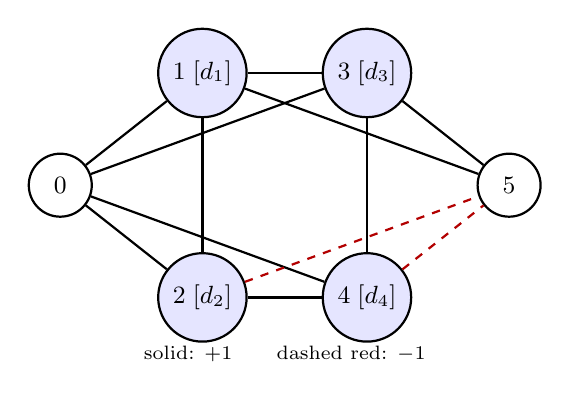
\begin{tikzpicture}[scale=.95,>=Latex,
  v/.style={circle,draw,thick,fill=white,minimum size=8mm,font=\small},
  p/.style={v,fill=blue!10}, posedge/.style={thick}, neg/.style={thick,dashed,red!70!black}]
\node[v] (s) at (-3,0) {$0$};
\node[p] (a) at (-1.1,1.5) {$1\;[d_1]$};
\node[p] (b) at (-1.1,-1.5) {$2\;[d_2]$};
\node[p] (c) at (1.1,1.5) {$3\;[d_3]$};
\node[p] (d) at (1.1,-1.5) {$4\;[d_4]$};
\node[v] (t) at (3,0) {$5$};
\foreach \x in {a,b,c,d}\draw[posedge] (s)--(\x);
\draw[posedge] (a)--(b); \draw[posedge] (a)--(c); \draw[posedge] (a)--(t);
\draw[posedge] (b)--(d); \draw[neg] (b)--(t);
\draw[posedge] (c)--(d); \draw[posedge] (c)--(t);
\draw[neg] (d)--(t);
\node[font=\scriptsize,align=left] at (0,-2.25) {solid: $+1$\qquad dashed red: $-1$};
\end{tikzpicture}

\caption{The locked six-state channel.  Solid lines carry (+1), dashed red
lines carry (-1), and the four internal vertices carry diagonal coordinates.}
\label{fig:model}
\end{figure}

\begin{proposition}[Baseline darkness]\label{prop:baseline-dark}
For \(d=0\), \(K(0,t)=0\) for every \(t\in\R\), equivalently
\(M_k(0)=0\) for every \(k\ge0\).
\end{proposition}
\begin{proof}
Let $S$ be either of the two signed involutions defined by the model.  It
satisfies $S^2=I$, $SH_0=H_0S$, $Se_0=e_0$ and
$e_5^{\mathsf T}S=-e_5^{\mathsf T}$.  Hence, for every $k$,
\[
M_k(0)=e_5^{\mathsf T}H_0^ke_0
=e_5^{\mathsf T}S H_0^k S e_0=-M_k(0),
\]
so $M_k(0)=0$ over characteristic zero.  Termwise substitution in the
globally convergent exponential series gives $K(0,t)=0$.
\end{proof}

\noindent\textbf{Formal status.}
The matrix identities, abstract signed-certificate implication and all-depth
conclusion are \evidence{KERNEL-CHECKED} as
\path{M3A.rOrig_involutive}, \path{M3A.rOrig_commutes_H0},
\path{M3A.selectedMoment_eq_zero_of_signedCertificate} and
\path{M3A.baseline_moments_dark}.  M8 checks the matrix-exponential passage;
no finite moment cutoff is used as a proof.

\begin{remark}
The proposition is about the channel, not about the persistence of any
particular certificate.  A perturbation may destroy a signed involution while
the transfer remains exactly zero for another reason.
\end{remark}

\section{Exact numerator and coefficient ideal}\label{sec:numerator}

Let \(\Delta(z;d)=\det(zI-H(d))\).  The selected adjugate cofactor is denoted
by \(N(z;d)\), so \(G=N/\Delta\) as a rational function before any common-factor
reduction.

\begin{theorem}[Exact selected numerator]\label{thm:numerator}
For the locked model,
\begin{equation}\label{eq:numerator}
\boxed{N(z;d)=L(z^2+2z)+2Q(z+1)+R.}
\end{equation}
This identity is \evidence{KERNEL-CHECKED} and independently
\evidence{VERIFIED-EXACT}.
\end{theorem}
\begin{proof}
Delete row \(0\) and column \(5\) from \(zI-H(d)\), take the determinant and
multiply by the cofactor sign \((-1)^{0+5}\).  In the Leibniz expansion, collect
terms by total diagonal degree.  The degree-one terms are
\(Lz^2+2Lz\); the degree-two terms are \(2Qz+2Q\); the degree-three terms are
\(R\); higher degrees cancel.  This gives \cref{eq:numerator}.  A second route
expands \(H(d)^k\), forms the Laurent series
\(G(z;d)=\sum_{k\ge0}M_k(d)z^{-k-1}\), and multiplies by the independently
computed denominator.  The release script performs both integer routes and
compares every monomial.
\end{proof}

\noindent\textbf{Formal status.}
The direct cofactor construction, retained row and column embeddings, cofactor
sign and universal identity over every commutative ring are checked by
\path{M3A.selectedMinor_eq_explicit} and
\path{M3A.selectedNumerator_formula}.  The determinant proof uses no sampled
evaluation or external symbolic output as a premise.

\begin{proposition}[Two-generator coefficient ideal]\label{prop:ideal}
Let \(\mathbb K\) be a field of characteristic different from \(2\),
equivalently a field in which \(2\) is invertible.  In
\(A=\mathbb K[d_1,d_2,d_3,d_4]\), the ideal of the coefficients of \(N\) is
\begin{equation}
I_N=(L,Q,R)=(L,Q).
\end{equation}
\end{proposition}
\begin{proof}
The coefficient list of \cref{eq:numerator} contains \(L\), \(2Q\) and \(R\),
so invertibility of \(2\) gives \(I_N=(L,Q,R)\).  The integral syzygy
\begin{equation}\label{eq:Rsyzygy}
R=-(d_2+d_4)Q-d_2d_4L.
\end{equation}
shows that \(R\in(L,Q)\), while \(L,Q\in I_N\) because \(L\) and \(2Q\) are
coefficients and \(2\) is a unit.  Hence equality.
\end{proof}

\noindent\textbf{Formal status.}
The coefficient syzygy and the implication $L=Q=0\Rightarrow R=0$ are
\evidence{KERNEL-CHECKED} as
\path{M3A.cubicNumeratorCoeff_syzygy} and
\path{M3A.cubicNumeratorCoeff_eq_zero_of_linear_quadratic_zero}.  The displayed
equality of ideals, as an equality in a multivariate polynomial ring, remains
a conventional algebraic proof rather than a theorem in the present Lean
package.

The exact-zero locus of the selected rational entry is therefore the algebraic
set \(V(L,Q)\), subject to no inference from a reduced numerator alone: the
identity is proved at the unreduced cofactor level.  Potential numerator--
denominator cancellation can lower a pole order, but cannot create a non-zero
rational entry when the unreduced numerator is the zero polynomial.

\begin{corollary}[Actual-coordinate transformed numerator]\label{cor:transformed}
With \(x=z^{-1}\),
\begin{equation}
x^{-1}G(x^{-1};d)=
\frac{Lx^3(1+2x)+2Qx^4(1+x)+Rx^5}{\Delta^\sharp(x;d)},
\end{equation}
where \(\Delta^\sharp(0;0)=1\).  Hence the denominator is a unit in the formal
local ring at \((x,d)=(0,0)\).
\end{corollary}

\section{Syzygy, dark planes and certificates}\label{sec:dark}

Define
\[
P_A=\{d_1=d_2,\ d_3=d_4\},\qquad
P_B=\{d_1=d_4,\ d_3=d_2\}.
\]

\begin{theorem}[Pointwise dark-plane decomposition]\label{thm:darkplanes}
Over every integral domain,
\begin{equation}\label{eq:darkpoints}
L(d)=Q(d)=0\quad\Longleftrightarrow\quad d\in P_A\cup P_B.
\end{equation}
On $P_A$ the original signed involution persists, and on $P_B$ the
alternative signed involution persists.  Consequently every selected moment,
and hence the selected amplitude, vanishes on the union.
\end{theorem}
\begin{proof}
Eliminate $d_1$ using $L=0$, so $d_1=d_2-d_3+d_4$.  Then
\[
Q=d_2d_4-(d_2-d_3+d_4)d_3=(d_2-d_3)(d_4-d_3).
\]
The absence of zero divisors gives either
$d_2=d_3$, $d_1=d_4$, which is $P_B$, or
$d_4=d_3$, $d_1=d_2$, which is $P_A$.  The converse follows by
substitution.  On each plane the matching diagonal perturbation commutes with
the stated signed involution, so the argument of
\cref{prop:baseline-dark} applies at every perturbation value.
\end{proof}

\noindent\textbf{Formal status.}
The equivalence \cref{eq:darkpoints} is \evidence{KERNEL-CHECKED} as
\path{M3A.ell_quad_zero_iff_planes}; Lean proves it over every integral domain.
The persistent commutators and the all-depth consequences are checked by
\path{M3A.rOrig_commutes_hamiltonian_of_planeA},
\path{M3A.rAlt_commutes_hamiltonian_of_planeB} and
\path{M3A.moments_dark_of_linear_quadratic_zero}.  M8 then gives actual
amplitude darkness.

\begin{proposition}[Reduced ideal decomposition]\label{prop:darkideal}
Over any field of characteristic different from $2$,
\begin{equation}\label{eq:darkdecomp}
(L,Q)=(d_1-d_2,d_3-d_4)\cap(d_1-d_4,d_3-d_2).
\end{equation}
Consequently the exact-dark scheme is the reduced union of two
two-dimensional linear planes.
\end{proposition}
\begin{proof}
The factorisation in the proof of \cref{thm:darkplanes} gives the two distinct
prime components after eliminating $L$.  Pulling them back to the original
polynomial ring gives \cref{eq:darkdecomp}; their intersection is radical.
\end{proof}

This scheme-theoretic ideal equality is \evidence{PROVED} in the paper but is
outside the current Lean scope.  Separating it from
\cref{thm:darkplanes} prevents the kernel-checked pointwise theorem from being
silently upgraded to an unformalised statement about polynomial ideals.

On a fixed ray $v=(a,b,c,d)$, the two planes read
\begin{equation}
P_A:\ a=b,\ c=d,\qquad P_B:\ a=d,\ c=b.
\end{equation}
They intersect in the scalar line $a=b=c=d$, an equality also checked in Lean
by \path{M3A.onPlaneA_and_onPlaneB_iff_scalarLine}.

\begin{figure}[ht]
\centering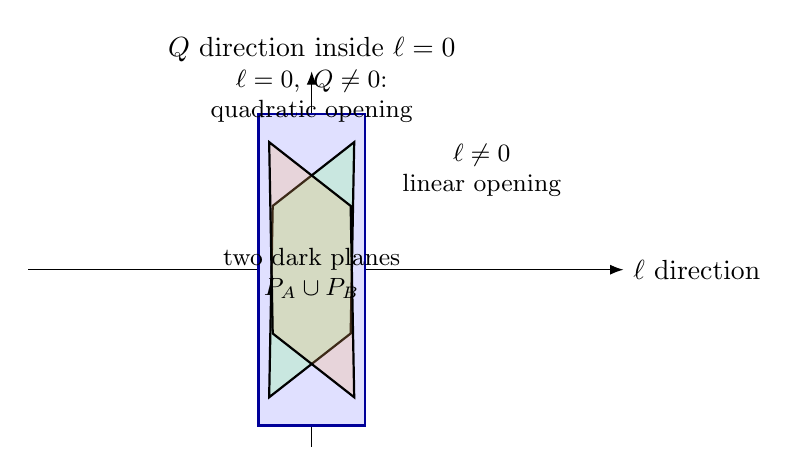
\begin{tikzpicture}[>=Latex,scale=.9,
  plane/.style={draw,thick,fill opacity=.24,text opacity=1},
  lab/.style={font=\small,align=center}]
\draw[->] (-4,0)--(4.4,0) node[right] {$\ell$ direction};
\draw[->] (0,-2.5)--(0,2.8) node[above] {$Q$ direction inside $\ell=0$};
\fill[blue!12] (-.75,-2.2) rectangle (.75,2.2);
\draw[blue!60!black,thick] (-.75,-2.2) rectangle (.75,2.2);
\draw[plane,fill=green!50] (-.6,-1.8)--(.55,-.9)--(.6,1.8)--(-.55,.9)--cycle;
\draw[plane,fill=orange!60] (-.55,-.9)--(.6,-1.8)--(.55,.9)--(-.6,1.8)--cycle;
\node[lab] at (2.4,1.4) {$\ell\ne0$\\linear opening};
\node[lab] at (0,2.45) {$\ell=0,\ Q\ne0$:\\quadratic opening};
\node[lab] at (0,-.05) {two dark planes\\$P_A\cup P_B$};
\end{tikzpicture}

\caption{Schematic direction stratification.  The ambient hyperplane
\(\ell=0\) contains the two exact-dark planes; points elsewhere on the
hyperplane have a quadratic opening.}
\label{fig:darkstrata}
\end{figure}

\subsection{Certificate discipline}

A signed involution $S$ with $SH_0=H_0S$, $Se_0=e_0$ and
$Se_5=-e_5$ is sufficient for baseline darkness.  Under perturbation the
commutator \([S,D(d)]\) may become non-zero.  This proves only that this
certificate has failed.  Exact opening requires a surviving coefficient of
$N$, of the moment series, or of $K$.  Conversely, a point of $V(L,Q)$
may be dark while failing to preserve a chosen presentation of $S$.

\begin{proposition}[Coefficient syzygy]\label{prop:syzygy}
The triple \((L,Q,R)\) satisfies the exact relation
\[
d_2d_4L+(d_2+d_4)Q+R=0.
\]
The relation explains why a nominal cubic numerator coefficient supplies no
third stratum after $L=Q=0$.
\end{proposition}

\begin{proof}
Expand the left-hand side and cancel the four cubic monomials.  This is
\cref{eq:Rsyzygy} rewritten and is also \evidence{KERNEL-CHECKED} as
\path{M3A.coefficient_syzygy}.
\end{proof}

This syzygy is the algebraic reason that the fixed-ray classification has only
linear, quadratic and exact-zero branches.  It is not a statement that the
cubic moment itself is generated by the two earlier moments; the tagged depth
information is addressed in \cref{sec:gf1}.

\section{Endpoint-access word support}\label{sec:endpoint}

The support restriction is clearest in a rectangular input--output setting.
Let
\[
A(\delta)=A_0+\sum_{r=1}^m\delta_rV_r,\qquad
M_k(\delta)=CA(\delta)^kB.
\]
For a multi-index \(\gamma\in\N^m\) with \(|\gamma|=j\), let
\(M_{\gamma,k}\) be the coefficient of \(\delta^\gamma\) in \(M_k\).
Define endpoint depths
\[
r_s(r)=\min\{q\ge0:V_rA_0^qB\ne0\},\qquad
r_t(r)=\min\{q\ge0:CA_0^qV_r\ne0\},
\]
with value \(\infty\) if the set is empty.  If a word realising \(\gamma\)
begins with label \(u\) at the source end and ends with label \(v\) at the
target end, call \((u,v)\) compatible.  Let
\[
\rho(\gamma)=\min_{(u,v)\ \mathrm{compatible}}
\bigl(r_s(u)+r_t(v)\bigr).
\]

\begin{theorem}[Endpoint-access bound]\label{thm:endpoint}
For \(j=|\gamma|\ge1\),
\begin{equation}\label{eq:endpointbound}
M_{\gamma,k}=0\quad\text{whenever}\quad k<j+\rho(\gamma).
\end{equation}
At \(k=j+\rho(\gamma)\), the coefficient is the sum of all compatible
endpoint-minimal words with zero internal gaps.  The bound is sharp if and only
if that boundary sum is non-zero.
\end{theorem}
\begin{proof}
Expand \(A(\delta)^k\) into labelled words.  A word contributing to
\(\delta^\gamma\) has \(j\) perturbation letters and \(k-j\) copies of \(A_0\).
If its first perturbation label at the source end is \(u\), at least
\(r_s(u)\) copies of \(A_0\) must lie to its right; if its last label at the
target end is \(v\), at least \(r_t(v)\) copies must lie to its left.  Internal
gaps are non-negative.  Therefore \(k-j\ge r_s(u)+r_t(v)\), and minimising gives
\cref{eq:endpointbound}.  Equality forces endpoint-minimal blocks and zero
internal gaps.  Summing all such words proves the boundary formula.  Distinct
words can cancel, so existence of words is not sharpness.
\end{proof}

The fully rectangular multi-index theorem above is \evidence{PROVED} by the
labelled-word argument.  The present Lean package formalises the locked
scalar-ray specialisation needed downstream, not this entire reusable
generality.

For the locked model \(B=e_0\), \(C=e_5^{\mathsf T}\), and
\(V_r=E_{rr}\) for \(r=1,\ldots,4\).  Every endpoint depth equals \(1\).

\begin{corollary}[Six-state support boundary]\label{cor:sixsupport}
For every \(\gamma\ne0\),
\[
[d^\gamma]M_k(d)=0\qquad(k<|\gamma|+2).
\]
At the minimal layer \(k=j+2\),
\begin{equation}\label{eq:minlayer}
\sum_{|\gamma|=j}[d^\gamma]M_{j+2}(d)d^\gamma
=d_1^j-d_2^j+d_3^j-d_4^j.
\end{equation}
Thus all mixed monomials vanish on the boundary.
\end{corollary}
\begin{proof}
The depth statement follows from the theorem.  On the boundary, the only word
is \(H_0D(d)^jH_0\), giving
\(e_5^{\mathsf T}H_0D(d)^jH_0e_0\).  Reading the four source and target edge
products in \cref{eq:H0} yields signs \(+,-,+,-\), proving
\cref{eq:minlayer}.
\end{proof}

\noindent\textbf{Formal status.}
For the locked channel, the complete finite word recurrence, the vanishing
below $k=j+2$, the boundary word and the signed power sum are
\evidence{KERNEL-CHECKED} as \path{M3A.rayCoeffMatrix},
\path{M3A.sixState_support_bound},
\path{M3A.rayMomentCoeff_boundary_matrix} and
\path{M3A.sixState_boundary_ray}.  These theorems sum actual word
coefficients, so boundary cancellation is already included.

The baseline \(j=0\) is deliberately excluded from the theorem: endpoint
depths are defined through a perturbation letter, and baseline darkness has its
own proof.  A finite census of 256 small labelled systems was used only to
stress-test common failure modes; it is \evidence{MEASURED} with \(n=256\), not
a proof of \cref{thm:endpoint}.

\section{Fixed-direction trichotomy}\label{sec:fixed}

Set \(v=(a,b,c,d)\in\R^4\) and \(H_v(\e)=H_0+\e D(v)\).  Define
\[
\ell=a-b+c-d,\qquad Q=bd-ac,\qquad
R=ab(c-d)+cd(a-b).
\]
The ray numerator is
\begin{equation}\label{eq:raynum}
N_v(z;\e)=\e\ell(z^2+2z)+2\e^2Q(z+1)+\e^3R.
\end{equation}

\begin{theorem}[Complete fixed-ray trichotomy]\label{thm:trichotomy}
Exactly one of the following holds.
\begin{enumerate}[label=(\alph*)]
\item If \(\ell\ne0\), the first perturbation/time pair is
      \((p,q)=(1,3)\), and the coefficient of \(\e t^3\) in \(K_v\) is
      \(i\ell/6\ne0\).
      Every other surviving exponent lies in
      \(((1,3)+\N^2)\setminus\{(1,3)\}\).
\item If \(\ell=0\) and \(Q\ne0\), then \((p,q)=(2,4)\), and the coefficient
      of \(\e^2t^4\) in \(K_v\) is \(Q/12\ne0\).
      Every other surviving exponent lies in
      \(((2,4)+\N^2)\setminus\{(2,4)\}\).
\item If \(\ell=Q=0\), then \(K_v(\e,t)\equiv0\); there is no cubic
      opening branch.
\end{enumerate}
\end{theorem}
\begin{proof}
The exact numerator \cref{eq:raynum} first separates the three cases.  If
\(\ell=Q=0\), the syzygy forces \(R=0\), so the rational entry and hence the
entire amplitude vanish.  For the first two cases, the endpoint support theorem
identifies the earliest possible time depth.  Direct boundary evaluation gives
\([\e]M_3=\ell\) and \([\e^2]M_4=2Q\).  Multiplication by
\((-i)^3/3!=i/6\) and \((-i)^4/4!=1/24\) gives the stated amplitude
coefficients.  Non-zero coefficients prove sharpness.
\end{proof}

\noindent\textbf{Formal status.}
The literal coefficient support and all three mutually exclusive branches are
\evidence{KERNEL-CHECKED} over complex directions by
\path{M3A.linearRayData_of_linear_ne},
\path{M3A.quadraticRayData_of_linear_zero_quadratic_ne},
\path{M3A.darkRayData_of_linear_quadratic_zero} and
\path{M3A.fixedRay_trichotomy}.  The claim that exactly one branch is selected
is additionally traced to \path{M3A.classifyRay_eq_linear_iff},
\path{M3A.classifyRay_eq_quadratic_iff},
\path{M3A.classifyRay_eq_dark_iff} and \path{M3A.classifyRay_spec}.  The exact
coefficient values are checked in M5, while M8 identifies the array with the
convergent matrix-exponential amplitude.  The real statement here follows by
scalar restriction.

The ordered pair \((p,q)\) is essential.  The numerator valuation \(p\) alone
does not encode time depth; \(q\) alone does not encode perturbative order.  For
the protected direction \(v_*=(1,0,-1,0)\), \(\ell=0\), \(Q=1\), and
the first amplitude coefficient is exactly (1/12).

\begin{corollary}[Dark rays]\label{cor:darkrays}
The fixed dark directions are precisely
\[
(a-b,c-d)=(0,0)\quad\text{or}\quad(a-d,c-b)=(0,0).
\]
\end{corollary}

\begin{remark}[Family-specific completeness]
The absence of a cubic branch is exact for this four-parameter diagonal family.
It is not a universal theorem for all analytic Hamiltonian perturbations.  A
two-state off-diagonal perturbation proportional to \(\e^3\) supplies an
immediate cubic-opening control.
\end{remark}

\section{Fixed-fibre Newton geometry}\label{sec:fixednewton}

For a fixed direction \(v\), let
\[
K_v(\e,t)=\sum_{p,q\ge0}A_{p,q}(v)\e^pt^q.
\]
Its Newton polyhedron is the convex hull of
\(\{(p,q):A_{p,q}(v)\ne0\}+\R_{\ge0}^2\).  Actual coefficients, rather than
candidate support, define this set.

\begin{theorem}[Fixed-fibre Newton polyhedra]\label{thm:fibrenewton}
For the three branches of \cref{thm:trichotomy}, the Newton polyhedron is,
respectively,
\[
(1,3)+\R_{\ge0}^2,\qquad
(2,4)+\R_{\ge0}^2,\qquad
\varnothing.
\]
Every positive weight exposes the unique displayed vertex in the non-dark
branches.
\end{theorem}
\begin{proof}
The trichotomy supplies the vertex and its non-zero coefficient.  The endpoint
bound shows that every other surviving exponent lies in the corresponding
upper orthant.  A strictly positive linear functional increases along every
non-zero vector in that orthant, hence exposes the vertex uniquely.
\end{proof}

\noindent\textbf{Formal status.}
The definition uses the actual non-zero coefficient support from M6 and the
Mathlib real convex hull.  The empty-germ convention, the general one-vertex
orthant lemma, the three fibre shapes and positive-weight uniqueness are
\evidence{KERNEL-CHECKED} as \path{M3A.newtonPolyhedron_empty},
\path{M3A.newton_eq_orthant_of_vertex},
\path{M3A.fixedFibre_newton} and
\path{M3A.fixedFibre_positiveWeight_faces}.

\begin{figure}[ht]
\centering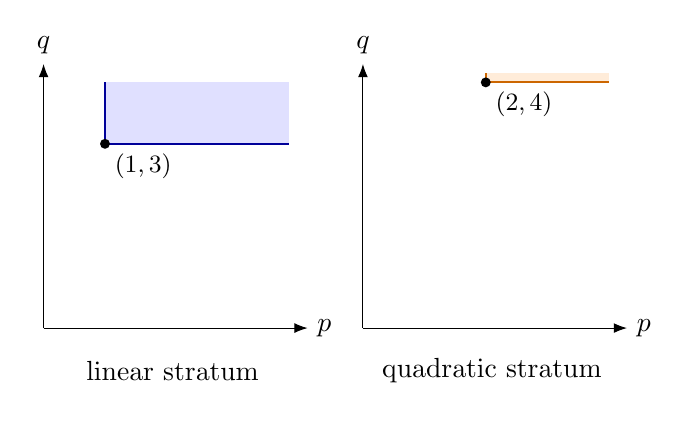
\begin{tikzpicture}[scale=.78,>=Latex]
\begin{scope}[xshift=-4.2cm]
\draw[->] (0,0)--(4.3,0) node[right] {$p$}; \draw[->] (0,0)--(0,4.3) node[above] {$q$};
\fill[blue!12] (1,3) rectangle (4,4); \fill[blue!12] (1,3) rectangle (4,3.25);
\draw[blue!60!black,thick] (1,3)--(4,3); \draw[blue!60!black,thick] (1,3)--(1,4);
\fill (1,3) circle (2.3pt); \node[below right,font=\small] at (1,3) {$(1,3)$};
\node at (2.1,-.7) {linear stratum};
\end{scope}
\begin{scope}[xshift=1cm]
\draw[->] (0,0)--(4.3,0) node[right] {$p$}; \draw[->] (0,0)--(0,4.3) node[above] {$q$};
\fill[orange!15] (2,4) rectangle (4,4.15); \draw[orange!80!black,thick] (2,4)--(4,4); \draw[orange!80!black,thick] (2,4)--(2,4.15);
\fill (2,4) circle (2.3pt); \node[below right,font=\small] at (2,4) {$(2,4)$};
\node at (2.1,-.7) {quadratic stratum};
\end{scope}
\end{tikzpicture}

\caption{Fixed-fibre Newton polyhedra.  The vertex moves from \((1,3)\) to
\((2,4)\) on the quadratic stratum; the exact-dark fibre has empty support.}
\label{fig:fixednewton}
\end{figure}

The change of variables \(x=z^{-1}\) in \cref{cor:transformed} is not cosmetic.
The resolvent expansion is a Laurent series at \(z=\infty\); multiplying by
\(x^{-1}\) aligns the coefficient of \(x^k\) with moment depth \(k\).  Omitting
that shift displaces every Newton point by one and corrupts the comparison with
the amplitude.

Classical Newton-polyhedron methods organise dominant exponents and exposed
faces \parencite{Kouchnirenko1976,Varchenko1976}.  Here the fibre theorem is
especially simple because there is one lower vertex.  The subtlety begins when
directions move or coordinates are pulled back, allowing several parent
exponents to collide.

\medskip
\noindent\textbf{Formalisation boundary.}
This completes the M0--M8 end-to-end Lean spine.  Beginning with
\cref{sec:pb1}, the paper moves to conventionally proved extensions supported
by exact symbolic or combinatorial checks.  No theorem in the remaining
sections is represented as part of the current Lean package unless explicitly
stated otherwise.

\section{Monomial pullback and face collision}\label{sec:pb1}

This section begins the extension beyond the current M0--M8 formalisation.
Its theorems are \evidence{PROVED} by the displayed finite-fibre arguments and
checked on released exact examples, but are not yet Lean theorems.

Let \(F(x)=\sum_{\alpha\in\N^n}A_\alpha x^\alpha\) be a formal series with
coefficients in a finite-dimensional vector space.  Fix an exponent matrix
\(\Lambda\in\N^{m\times n}\) with no zero column and non-zero leading constants
\(c_i\).  Define
\[
x_i=c_i y^{\lambda_i},\qquad
\lambda_i\in\N^m.
\]

\begin{theorem}[Fibre aggregation]\label{thm:aggregation}
The pulled coefficient at child exponent \(\beta\) is
\begin{equation}\label{eq:aggregation}
B_\beta(c)=\sum_{\Lambda\alpha=\beta}A_\alpha c^\alpha.
\end{equation}
The sum is finite.  Hence the actual child support is contained in, but may be
strictly smaller than, the naive image \(\Lambda(\supp F)\).
\end{theorem}
\begin{proof}
Substitution gives
\(A_\alpha c^\alpha y^{\Lambda\alpha}\).  Group equal child monomials to obtain
\cref{eq:aggregation}.  If \(\Lambda\alpha=\beta\), then for every column choose
a positive entry; this bounds each \(\alpha_i\) by a coordinate of \(\beta\),
so the fibre is finite.  Its sum can cancel.
\end{proof}

For a positive child weight \(\mu\), set \(w=\Lambda^{\mathsf T}\mu\) and let
\(\phi^{\rm gr}\) denote substitution by leading monomials.
This valuation transport is adjacent to tropical elimination
\parencite{SturmfelsTevelev2008}; the coefficient-fibre cancellation test is
kept explicit because equations can retain information lost by set-theoretic
support alone \parencite{Giansiracusa2016}.

\begin{theorem}[Candidate face and equality criterion]\label{thm:pullbackface}
If \(\nu_w(F)\) is the parent valuation, then
\[
\nu_\mu(\phi F)\ge\nu_w(F).
\]
The candidate component at that weight is
\begin{equation}\label{eq:candidateface}
\phi^{\rm gr}(\inw_w F).
\end{equation}
Equality holds if and only if \cref{eq:candidateface} is non-zero.  A literal
identity \(\inw_\mu(\phi F)=\phi^{\rm gr}(\inw_wF)\) without the non-vanishing
hypothesis is \evidence{FALSIFIED}.
\end{theorem}
\begin{proof}
Every parent monomial has child weight
\(\mu\cdot\Lambda\alpha=w\cdot\alpha\), so no pulled term can have smaller
weight.  Aggregating all parent terms of minimal weight gives
\cref{eq:candidateface}.  If it survives, it is the child initial form.  If it
cancels, the actual valuation is larger and the displayed right-hand side is
zero, whereas the child initial form, when the pullback is non-zero, occurs at a
later weight.
\end{proof}

\begin{figure}[ht]
\centering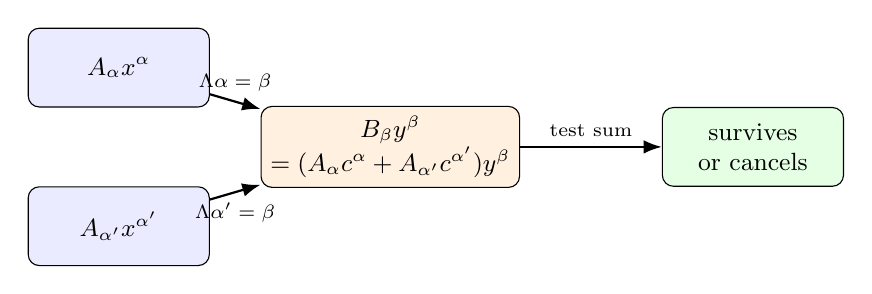
\begin{tikzpicture}[>=Latex,node distance=10mm and 18mm,
  box/.style={draw,rounded corners,minimum width=23mm,minimum height=10mm,align=center,font=\small},
  arr/.style={->,thick}]
\node[box,fill=blue!8] (a) {$A_\alpha x^\alpha$};
\node[box,fill=blue!8,below=of a] (ap) {$A_{\alpha'}x^{\alpha'}$};
\node[box,fill=orange!12,right=of $(a)!0.5!(ap)$] (b) {$B_\beta y^\beta$\\$=(A_\alpha c^\alpha+A_{\alpha'}c^{\alpha'})y^\beta$};
\node[box,fill=green!10,right=of b] (decision) {survives\\or cancels};
\draw[arr] (a)--node[above,font=\scriptsize] {$\Lambda\alpha=\beta$} (b);
\draw[arr] (ap)--node[below,font=\scriptsize] {$\Lambda\alpha'=\beta$} (b);
\draw[arr] (b)--node[above,font=\scriptsize] {test sum} (decision);
\end{tikzpicture}

\caption{Two parent exponents can enter the same child fibre.  Their aggregate,
not their separate presence, decides the child support.}
\label{fig:pullback}
\end{figure}

Under successive monomial maps with exponent matrices \(\Lambda\) then
\(\Omega\), exponents compose as \(\Omega\Lambda\); leading constants compose
as \(c_i d^{\lambda_i}\).  After a cancellation, however, the next survivor can
depend on the full germ and on unit jets, not merely on the first exponent
matrix.  No universal ``next face'' rule from the cancelled face alone is
claimed.

\section{Analytic-arc valuation}\label{sec:arc1}

Let \(v(\eta)=(a(\eta),b(\eta),c(\eta),d(\eta))\) be an analytic germ and set
\[
\alpha=\ord_\eta\ell(v(\eta)),\qquad
\beta=\ord_\eta Q(v(\eta)),
\]
with order \(\infty\) for the zero germ.  The three-scale pullback is
\(\e=c_\e s^b\), \(t=c_t s^a\), \(\eta=c_\eta s^c\), with
positive exponents \(a,b,c\) and non-zero constants.

\begin{theorem}[Analytic-arc lower hull]\label{thm:arc}
The only candidate lower points are
\[
P_\ell=(1,3,\alpha),\qquad P_Q=(2,4,\beta),
\]
omitting a point whose order is \(\infty\).  Their pulled costs are
\[
\kappa_\ell=b+3a+c\alpha,\qquad
\kappa_Q=2b+4a+c\beta.
\]
The lower hull is classified as follows:
\begin{enumerate}[label=(\roman*)]
\item if \(\alpha\le\beta<\infty\), \(P_\ell\) dominates;
\item if \(\beta<\alpha<\infty\), both points are vertices, with a tie on
      \(c(\alpha-\beta)=a+b\);
\item if \(\alpha=\infty\) and \(\beta<\infty\), only \(P_Q\) remains;
\item if \(\alpha=\beta=\infty\), the arc is exactly dark.
\end{enumerate}
\end{theorem}
\begin{proof}
The endpoint theorem gives \(q\ge p+2\) for every positive perturbation degree
\(p\); the \(p=0\) layer is zero by baseline darkness.  Every positive-degree
coefficient polynomial vanishes on the exact-dark locus.  Since
\((L,Q)\) is radical by \cref{prop:darkideal}, each such coefficient belongs to
\((L,Q)\).  More sharply, complete first-order protection shows that every
\(p=1\) coefficient lies in \((L)\).  After restriction to the analytic arc,
a \(p=1\) term therefore has order at least \(\alpha\) and cost at least
\(b+3a+c\alpha=\kappa_\ell\).

For \(p\ge2\), coefficient membership in \((L,Q)\) gives order at least
\(\min(\alpha,\beta)\), while endpoint support gives cost at least
\[
pb+(p+2)a+c\min(\alpha,\beta).
\]
If \(\alpha\le\beta\), this exceeds \(\kappa_\ell\) by at least \(a+b\).
If \(\beta<\alpha\), it is at least \(\kappa_Q\), with equality possible only
at the displayed \((2,4,\beta)\) boundary candidate.  Thus no hidden
higher-order coefficient can lie below the two stated candidates.  Comparing
their costs gives
\(\kappa_\ell-\kappa_Q=c(\alpha-\beta)-(a+b)\), which yields the four cases.
If both germs vanish, every positive-degree coefficient vanishes by membership
in \((L,Q)\), while the baseline layer is already dark; hence the whole arc is
exactly dark.
\end{proof}

On a tie, write \(\ell=\ell_\alpha\eta^\alpha+\cdots\) and
\(Q=Q_\beta\eta^\beta+\cdots\).  The candidate amplitude coefficient is
\begin{equation}\label{eq:tiecoef}
\frac{i\ell_\alpha c_\e c_\eta^\alpha c_t^3}{6}
+\frac{Q_\beta c_\e^2c_\eta^\beta c_t^4}{12}.
\end{equation}

\begin{proposition}[Field-corrected tie rule]\label{prop:tiefield}
Over \(\C\), the tied coefficient can cancel at
\begin{equation}\label{eq:ctcancel}
c_t=-\frac{2i\ell_\alpha c_\eta^{\alpha-\beta}}{Q_\beta c_\e}.
\end{equation}
For a real-analytic Hermitian family with real
\(\ell_\alpha,Q_\beta,c_\e,c_\eta,c_t\ne0\), the two terms in
\cref{eq:tiecoef} have orthogonal real and imaginary parts and cannot cancel.
No real non-cancellation statement is made for complex leading data.
\end{proposition}
\begin{proof}
Factor the non-zero cubic term from \cref{eq:tiecoef}; the remaining affine
factor in \(c_t\) gives \cref{eq:ctcancel}.  Under the stated real hypotheses,
the first summand is purely imaginary and the second purely real.
\end{proof}

\begin{figure}[ht]
\centering\begin{tikzpicture}[scale=.9,>=Latex]
\draw[->] (0,0)--(5,0) node[right] {$p$};
\draw[->] (0,0)--(0,4.4) node[above] {$q$};
\draw[->] (0,0)--(-1.8,-1.4) node[below left] {$\eta$-order};
\coordinate (L) at (1.1,3.1); \coordinate (Q) at (3.4,2.0);
\draw[very thick,blue!60!black] (L)--(Q);
\fill[blue!70!black] (L) circle (2.6pt); \fill[orange!80!black] (Q) circle (2.6pt);
\node[above left,font=\small] at (L) {$P_\ell=(1,3,\alpha)$};
\node[below right,font=\small] at (Q) {$P_Q=(2,4,\beta)$};
\draw[red!70!black,thick,dashed] (-.3,3.85)--(4.35,1.15);
\node[red!70!black,font=\small,rotate=-30] at (3.3,3.15) {tie weight plane};
\end{tikzpicture}

\caption{The two analytic-arc candidates.  A weight plane can expose one point
or their joining edge; coefficient cancellation is a separate test on that
edge.}
\label{fig:arclower}
\end{figure}

\subsection{A tie and its next survivor}

Take \(v(\eta)=(1+\eta^2,0,-1,0)\), so \(\alpha=2\), \(\beta=0\), and use
equal scale exponents.  At total order six,
\[
[s^6]K=\frac{c_\e^2c_t^4}{12}+\frac{i c_\e c_t^3}{6}.
\]
With \(c_\e=1,c_t=-2i\), this cancels.  Exact expansion gives
\[
[s^7]K=\frac{c_\e c_t^4}{12}-\frac{i c_\e^2c_t^5}{60}=\frac45.
\]
The survivor \(4/5\) is \evidence{VERIFIED-EXACT}.  Its value cannot be inferred
from \((\alpha,\beta)\) alone; it uses later coefficients of the pulled germ.

Regular analytic reparametrisation preserves \(\alpha,\beta\) and leading
scales.  A singular reparametrisation \(\eta=\xi^r\) multiplies both finite
orders by \(r\).  Analyticity is essential: the smooth-flat germ
\(e^{-1/\eta^2}\) has zero Taylor series at the origin without vanishing on a
punctured neighbourhood.

Finally, if an analytic arc is dark, the product factorisation on \(L=0\) and
the integral-domain property of convergent power-series rings show that the
whole germ lies in one of the two dark components.  It cannot switch components
infinitely often near the origin while remaining analytic.

\section{Universal multivariate Newton atlas}\label{sec:mv1}

Return to the actual coordinates \(d_1,\ldots,d_4,t\).  By
\cref{cor:sixsupport}, every non-zero moment monomial \(d^\gamma t^k\) with
\(\gamma\ne0\) satisfies \(k\ge|\gamma|+2\), and the boundary consists only of
pure powers.

\begin{theorem}[Universal Newton polyhedron]\label{thm:universalnewton}
The Newton polyhedron of \(K(d,t)\) at the dark origin is
\begin{equation}\label{eq:universalNP}
\conv\{(e_1,3),(e_2,3),(e_3,3),(e_4,3)\}+\R_{\ge0}^{5}.
\end{equation}
At the four vertices the raw moment coefficients are \(+1,-1,+1,-1\), and the
amplitude coefficients are \(i/6,-i/6,i/6,-i/6\).
\end{theorem}
\begin{proof}
For \(\gamma=0\), all coefficients vanish by the all-depth baseline-darkness
theorem, so no unperturbed exponent enters the universal support.  The
\(j=1\) case of \cref{eq:minlayer} supplies the four non-zero vertices.  For
any other exponent \((\gamma,k)\) with \(\gamma\ne0\), choose \(r\) with
\(\gamma_r>0\).  Then \(k\ge|\gamma|+2\ge3\), and
\((e_r,3)\le(\gamma,k)\) coordinatewise.  Hence all actual support lies in the
upper closure of the four vertices.  The amplitude coefficients follow from
\((-i)^3/3!=i/6\).
\end{proof}

For a positive weight \(\omega=(\omega_1,\ldots,\omega_4,\tau)\), the exposed
vertices are indexed by the non-empty subset
\[
I(\omega)=\{r:\omega_r=\min_j\omega_j\}.
\]
Every non-empty subset occurs, giving exactly \(2^4-1=15\) relatively open
cells.  On a cell \(I\), the face polynomial is
\begin{equation}\label{eq:mvface}
\frac{i}{6}t^3\sum_{r\in I}\sigma_r d_r,\qquad
(\sigma_1,\sigma_2,\sigma_3,\sigma_4)=(1,-1,1,-1).
\end{equation}
Over the complex torus, every face with at least two vertices has a cancellation
hypersurface.  Over the positive real torus, a face cancels only when \(I\)
contains both signs.

\begin{figure}[ht]
\centering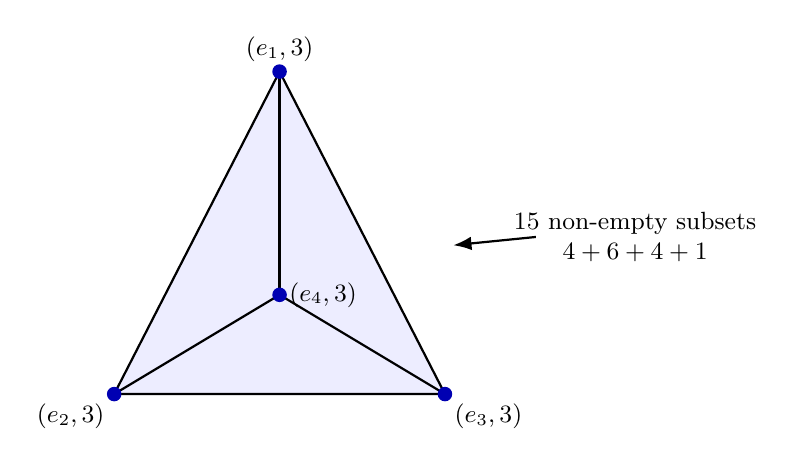
\begin{tikzpicture}[scale=1.05,>=Latex]
\coordinate (A) at (0,2.8); \coordinate (B) at (-2,-1.1); \coordinate (C) at (2,-1.1); \coordinate (D) at (0,.1);
\fill[blue!7] (A)--(B)--(C)--cycle;
\draw[thick] (A)--(B)--(C)--cycle; \draw[thick] (A)--(D)--(B); \draw[thick] (D)--(C);
\draw[dashed] (B)--(C); \draw[thick] (D)--(A);
\fill[blue!70!black] (A) circle (2.5pt); \node[above,font=\small] at (A) {$(e_1,3)$};
\fill[blue!70!black] (B) circle (2.5pt); \node[below left,font=\small] at (B) {$(e_2,3)$};
\fill[blue!70!black] (C) circle (2.5pt); \node[below right,font=\small] at (C) {$(e_3,3)$};
\fill[blue!70!black] (D) circle (2.5pt); \node[right,font=\small] at (D) {$(e_4,3)$};
\node[align=center,font=\small] at (4.3,.8) {$15$ non-empty subsets\\$4+6+4+1$};
\draw[->,thick] (3.1,.8)--(2.1,.7);
\end{tikzpicture}

\caption{A tetrahedral projection of the four Newton vertices.  Its non-empty
vertex subsets encode the 15 positive normal cells; this is a combinatorial
projection, not a Euclidean embedding of the five-dimensional polyhedron.}
\label{fig:mv1cells}
\end{figure}

\subsection{Moment--amplitude face mismatch}

The moment and amplitude have the same exponent support, because the multiplier
\((-i)^k/k!\) is never zero.  Their face cancellation equations need not agree
when a pullback makes distinct time depths tie.  A reachable two-term face with
parent points \((e_1,4)\) and \((e_2,3)\) has raw coefficients \(2,-1\).  Its
moment and amplitude face forms are
\[
W_M=2c_1-c_2,\qquad W_A=\frac{c_1}{12}-\frac{i c_2}{6}.
\]
Thus equality of supports does not imply equality of cancellation loci.

\subsection{Fixed positive rational weights}

The following corrects an overly pessimistic interpretation of the finite
universal atlas obstruction.

\begin{theorem}[Fixed-weight coefficient-stratified termination]\label{thm:noetherian}
For every fixed positive rational weight, after finite ramification where
needed, the pulled amplitude has a finitely generated coefficient ideal, so a
finite coefficient-stratified exact-zero/first-survivor decision exists.  No
effective uniform depth bound or finite global recursive atlas over all
positive weights has been proved.
\end{theorem}
\begin{proof}
Clear denominators in the fixed rational weight by a ramification \(s=u^m\).
After substituting
\(d_r=c_ru^{b_r}\) and \(t=c_tu^a\), write the pulled amplitude as
\[
K_\omega(u;c)=\sum_{n\ge0}A_n(c)u^n,
\]
where each \(A_n\) is a polynomial in the leading constants over the base field
(or a Laurent polynomial if constants are restricted to the torus).  The ring
\(\mathbb K[c_1,\ldots,c_4,c_t]\), and likewise its Laurent localisation, is
Noetherian \parencite{AtiyahMacdonald1969}.  Therefore the ideal
\(J=(A_n:n\ge0)\) is generated by a finite subset, say with indices at most
\(N\).  If \(A_0(c)=\cdots=A_N(c)=0\), then every \(A_n(c)=0\), so the pullback
is exactly zero.  Otherwise its first survivor occurs among those finitely many
indices.  This proves existence for the fixed weight.  The argument neither
computes a useful \(N\) nor bounds \(N\) uniformly as the weight varies.
\end{proof}

The theorem concerns a coefficient-stratified decision, not a weight-only
decision.  Delayed cancellations can make the necessary depth arbitrarily
large across families of weights or germs; that fact is compatible with
Noetherianity at each fixed weight.

\section{Gr\"obner, Rees and marked-channel structures}\label{sec:gf1}

The dark ideal \(I=(L,Q)\) records exact zero sets but forgets which generator
enters at which perturbation and time depth.  The following hierarchy makes the
information loss explicit.

Introduce adapted coordinates
\[
\lambda=L,\qquad \xi=d_2-d_3,\qquad \eta=d_4-d_3,\qquad \zeta=d_3.
\]
Then
\[
d_1=\lambda+\xi+\eta+\zeta,\quad d_2=\xi+\zeta,
\quad d_3=\zeta,\quad d_4=\eta+\zeta
\]
and
\begin{equation}\label{eq:normalcrossing}
Q=\xi\eta-\lambda\zeta,\qquad I=(\lambda,\xi\eta)
=(\lambda,\xi)\cap(\lambda,\eta).
\end{equation}
Thus the two components meet normally inside the hyperplane \(\lambda=0\), but
their union has codimension two in the ambient four-space; calling it an
ambient normal-crossing divisor would be incorrect.

\begin{theorem}[Gr\"obner fan of the dark ideal]\label{thm:fan}
In the original coordinates the dark ideal has 16 full-dimensional monomial
initial cones.  Twelve initial ideals are radical squarefree intersections of
two planes.  Four are doubled planes:
\[
(d_1,d_3^2),\quad(d_2,d_4^2),\quad(d_3,d_1^2),\quad(d_4,d_2^2).
\]
Every cone has dimension \(2\), degree \(2\), Hilbert series
\((1+t)/(1-t)^2\) and Hilbert polynomial \(2n+1\).  Initialisation commutes with
the two-component intersection in exactly the twelve radical cones.
\end{theorem}
\begin{proof}
Run Buchberger reduction for each strict ordering chamber of the four variables,
merge chambers with the same reduced marked basis, and retain the 16 distinct
initial ideals.  Monomial primary decomposition gives the twelve squarefree and
four primary cases.  Counting standard monomials yields the common Hilbert
series and polynomial.  The complete marked bases, representative weights,
facets and adjacency graph are reproduced in \cref{app:atlases}.  An independent
exact script checks the counts and invariants against the released JSON atlas.
\end{proof}

\begin{proposition}[Rees algebra]\label{prop:rees}
Let \(Y_L,Y_Q\) mark the two generators.  Then
\[
\mathcal R(I)\cong
\frac{A[Y_L,Y_Q]}{(QY_L-LY_Q)}.
\]
The ideal is of linear type and its powers are integrally closed.  The blow-up
does not separate the two dark components: its exceptional geometry retains a
singular section over their intersection.
\end{proposition}
\begin{proof}
The two generators form a regular sequence in the polynomial ring, so the Rees
kernel is generated by the Koszul relation \(QY_L-LY_Q\).  In the adapted
normal form \((\lambda,\xi\eta)\), the Newton polyhedron of each monomial power
is saturated in its exponent lattice, giving integral closure.  The two affine
blow-up charts follow by setting either Rees coordinate to one; their equations
retain the component-intersection section.
\end{proof}

For an arc with orders
\(a=\ord\lambda\), \(b=\ord\xi\), \(c=\ord\eta\), its basic contact profile is
\begin{equation}\label{eq:contact}
\bigl(\min(a,b+c),\min(a,c),\min(a,b),\min(a,b,c)\bigr).
\end{equation}
Arc-space contact loci provide the general geometric context
\parencite{Ein2004}; \cref{eq:contact} is the exact specialised formula.

\subsection{Tagged ideal and marked section}

Introduce tags \(u\) for perturbation order and \(x\) for time depth.  The
tagged channel ideal is
\begin{equation}
J=(Lu x^3,\;Qu^2x^4,\;Ru^3x^5)=(Lu x^3,Qu^2x^4),
\end{equation}
with first syzygy \((Qux,-L)\).  Saturating away the tags recovers the dark
ideal, but the plain ideal cannot reconstruct the tags.

Let a free module have basis \(e_L,e_Q,e_R\).  The numerator marking is
\[
s_N=(1+2x)e_L+2(1+x)e_Q+e_R,
\]
and the kernel includes
\[
(Qux,-L,0),\qquad(d_2d_4u^2x^2,(d_2+d_4)ux,1).
\]
The first records the two-generator relation with depth tags; the second records
the cubic syzygy.  Even this marked numerator section is not the full amplitude:
denominator inversion and factorial phases remain necessary.

\begin{figure}[ht]
\centering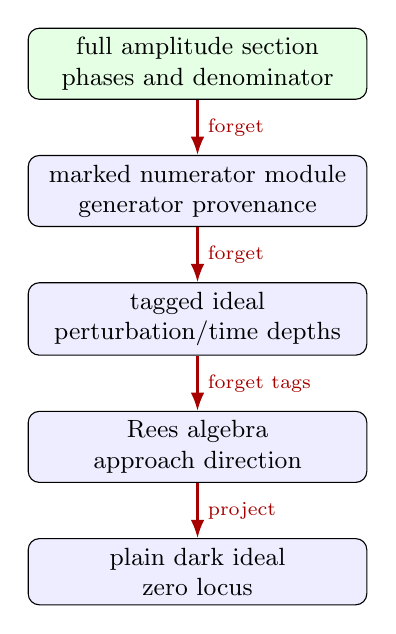
\begin{tikzpicture}[node distance=7mm,>=Latex,
  box/.style={draw,rounded corners,fill=blue!7,minimum width=43mm,minimum height=8mm,align=center,font=\small},
  arr/.style={->,thick,red!65!black}]
\node[box,fill=green!10] (amp) {full amplitude section\\phases and denominator};
\node[box,below=of amp] (marked) {marked numerator module\\generator provenance};
\node[box,below=of marked] (tag) {tagged ideal\\perturbation/time depths};
\node[box,below=of tag] (rees) {Rees algebra\\approach direction};
\node[box,below=of rees] (plain) {plain dark ideal\\zero locus};
\draw[arr] (amp)--node[right,font=\scriptsize]{forget} (marked);
\draw[arr] (marked)--node[right,font=\scriptsize]{forget} (tag);
\draw[arr] (tag)--node[right,font=\scriptsize]{forget tags} (rees);
\draw[arr] (rees)--node[right,font=\scriptsize]{project} (plain);
\end{tikzpicture}

\caption{Information hierarchy.  Moving left is a lossy forgetful operation;
the plain dark ideal cannot recover depth tags or amplitude phases.}
\label{fig:hierarchy}
\end{figure}

For the mixed path \(d=(s,s^3,-s,s^4)\), a tied face has
\[
W_M=-c^3+2c^4,\qquad W_A=-\frac{i c^3}{6}+\frac{c^4}{12}.
\]
At \(c=2i\), the amplitude face cancels and the exact next coefficient is
\(-32/15\) at order seven.  This control is \evidence{VERIFIED-EXACT} and
exhibits why the full amplitude section is the terminal object in the hierarchy.

\section{Counterexamples and scope firewalls}\label{sec:scope}

The framework is defined as much by its negative results as by its exact
theorems.  The following controls block tempting but false upgrades.

\begin{longtable}{p{0.24\textwidth}p{0.30\textwidth}p{0.36\textwidth}}
\toprule
Tempting inference & Exact control & Correct conclusion\\
\midrule
\endhead
Broken certificate \(\Rightarrow\) opening & A perturbation can destroy a
chosen involution while remaining in \(V(L,Q)\). & Certificate failure is not a
surviving transfer coefficient.\\
Closure \(\Rightarrow\) certificate & Krylov closure is an invariant-subspace
property. & It need not supply a signed involution.\\
Candidate support \(\Rightarrow\) child support & Two parent exponents can
share a monomial fibre and cancel. & Aggregate by \cref{eq:aggregation} first.\\
Initial form always commutes with pullback & A cancelled candidate face has
zero graded pullback but a later non-zero child initial form. & The equality
needs the non-vanishing criterion of \cref{thm:pullbackface}.\\
Moment face \(=\) amplitude face & The reachable forms
\(2c_1-c_2\) and \(c_1/12-ic_2/6\) have different zeros. & Support agrees;
cancellation can differ.\\
Real tie cannot cancel & Equation \cref{eq:ctcancel} cancels over \(\C\). & Real
non-cancellation needs real-analytic Hermitian data and real constants.\\
The cubic numerator creates a third branch & \(R=-(d_2+d_4)Q-d_2d_4L\). & No
cubic fixed-ray branch exists in this family.\\
No cubic opening exists at all & A two-state family with off-diagonal coupling
\(\e^3\) opens cubically. & The trichotomy is family-specific.\\
Plain ideal retains depth & \((L,Q)\) is unchanged after tags are forgotten. &
Use the tagged ideal or marked section.\\
Blow-up separates the two components & The Rees charts retain a singular
section over the intersection. & Blow-up records approach data but does not
separate these components.\\
Finite fixed-weight decision \(\Rightarrow\) uniform atlas & Noetherianity
chooses generators after the weight is fixed. & No effective uniform depth or
finite global recursive atlas is proved.\\
Smooth-flat order \(\infty\) \(\Rightarrow\) zero germ &
\(e^{-1/\eta^2}\) is flat but non-zero away from \(0\). & The analytic-arc
theorem is not a smooth-germ theorem.\\
One formalised theorem \(\Rightarrow\) the whole paper is formalised & M0--M8
stop at the fixed-fibre analytic bridge. & Use the named theorem map and treat
the later extensions as conventionally proved.\\
\bottomrule
\end{longtable}

\begin{counterexample}[The symbol \(R\) is not the cubic moment]
For \(v=(1,0,0,0)\), the cubic numerator coefficient \(R(v)\) is zero, while
the relevant cubic moment coefficient is \(1\).  Algebraic numerator degree and
time depth are distinct gradings.
\end{counterexample}

\begin{counterexample}[Scalar rays lose the universal fan]
The substitution \(d=\e v\) collapses the four coordinate vertices to a single
perturbation coordinate.  It therefore cannot retain the 15-cell normal atlas
of \cref{thm:universalnewton}.  Fixed rays and actual coordinates answer
different questions.
\end{counterexample}

\subsection{Publication scope}

The exact claims concern the locked matrix \cref{eq:H0}, its four internal
diagonal coordinates, formal or analytic local expansions, and declared real
or complex coefficient domains.  They do not establish robustness under
dissipation, experimental noise, arbitrary graph size, arbitrary perturbation
support, or a canonical physical interpretation of a multi-Rees construction.
Connections to quantum transport, dark states and tropical geometry are
positioning links, not priority claims.  The priority of the full exact
synthesis in the literature is \evidence{UNAVAILABLE}; the prior-art audit found
no matching theorem but did not prove absence.

The formal claim is narrower and auditable: only the statements listed in
\cref{tab:leanmap,app:reprochecks} are \evidence{KERNEL-CHECKED}.  This boundary
is about proof status, not mathematical importance; it does not weaken the
conventional proofs in the extension sections, nor promote their exact scripts
to formal proofs.

\section{Formal verification, reproducibility and transparency}
\label{sec:repro}

The release separates kernel checking, conventional proof, exact computation,
byte identity and measurement.  The formal project is the primary executable
evidence for the M0--M8 spine.  Exact integer and rational scripts remain
independent regression checks for the locked numerator, denominator, moment
boundary, arc controls and atlas invariants.  No floating-point tolerance
enters a theorem certificate.

\subsection{Lean build and trust report}

The formalisation pins both Lean and Mathlib to version 4.32.1.  Its root module
imports \path{M3A.AnalyticBridge}, which transitively imports every earlier
stage.  A clean \path{lake build} completed successfully after M8.  The
principal axiom reports contain only \path{propext},
\path{Classical.choice} and \path{Quot.sound}; there is no
\path{sorry}, \path{admit}, user-declared axiom or unsafe theorem dependency.
The theorem-level map is reproduced in \cref{app:reprochecks}.

This trust statement follows the standard Lean architecture
\parencite{deMouraUllrich2021}: tactics and automation may construct proof
terms, but acceptance of those terms is checked by the kernel.  Mathlib
provides the matrix, power-series, topology and convexity infrastructure used
in the development \parencite{MathlibCommunity2020}.  Neither citation is used
as evidence for the M3A theorems themselves; their evidence is the released
source and checked proof terms.

\subsection{Independent exact routes}

\begin{enumerate}[label=\arabic*.]
\item \textbf{Lean route.}  Finite matrix definitions, cofactor expansion,
      word recurrence, support classification, convex hull and analytic
      summation form one checked dependency chain.
\item \textbf{Cofactor route.}  A direct Leibniz determinant gives (N) and the
      52-term denominator.
\item \textbf{Moment route.}  Polynomial matrix powers give $M_k$, endpoint
      support and the signed minimal layer.
\item \textbf{Pulled-amplitude route.}  Gaussian-rational series compute the
      ARC1 and GF1 tie cancellations and next survivors.
\item \textbf{Combinatorial route.}  Released JSON atlases are checked for all
      15 MV1 cells and all 16 GF1 cones, including radicality flags and Hilbert
      data.
\end{enumerate}
The cofactor and moment routes meet at the Laurent expansion of the resolvent;
agreement is a cross-check, not circular evidence.  Although finite
Hamiltonian entries generate highly structured series, no general D-finite
closure claim is needed here \parencite{Stanley1980}.

\subsection{Executable discrepancy fixture}

The fixture changes the symmetric edge pair
$H_{0,2}=H_{2,0}=-1$ to $+1$.  It then reruns the same cofactor and moment
code.  Both routes detect disagreement with the locked numerator and moment
layer.  The fixture result is computed at run time and written to
\path{DATA/discrepancy_detection.json}; it is not a stored truth value.

\subsection{Source recovery}

The workstation scan hashed 3,636 scientific-source files and found 932 unique
byte streams, including 631 duplicate-content groups.  It searched 780 unique
text streams and extracted 20 unique PDFs without a read failure.  Those counts
are \evidence{MEASURED} with the stated sample sizes.  Vendor TeX
distributions, dependency caches, rendered scratch files and the output tree
were excluded and recorded.  Byte-identical copies were searched once and
linked by SHA-256; filename suffixes such as ``copy'' or parenthetical numbers
were not treated as authority.

\paperone{} has the verified Zenodo version DOI
\href{https://doi.org/10.5281/zenodo.20556571}{10.5281/zenodo.20556571} and is
cited accordingly \parencite{MedfordPaperI}.  Its source is available in the
\href{https://github.com/SLresearch74/Signed-Involution-Sector-Exclusion-for-EZT-in-Finite-Magnetic-Graph-Hamiltonians---v1.0.0}{public GitHub repository}.
The Zenodo record is version \path{v1.0.0}; as of 10 August 2026 the GitHub
repository has no separate Release or tag.  Paper II reproducibility materials
are located under
\path{subsequent-work/paper-2-opening-theory/} in that repository.  The earlier
R1.2 Paper II manuscript remains an author-supplied unpublished preprint with
no invented identifier.

\subsection{How to reproduce}

From the formalisation root, run
\begin{verbatim}
lake build
lake env lean M3AFormalisation.lean
\end{verbatim}
From \path{subsequent-work/paper-2-opening-theory}, run
\begin{verbatim}
python CODE/verify_paper.py
python CODE/verify_paper.py --fixture
cd paper/source
latexmk -pdf -interaction=nonstopmode -halt-on-error main.tex
\end{verbatim}
The paper build uses Biber for Harvard author--date citations.  Exact
environment versions, milestone verification reports, expected JSON and the
release manifest accompany the source.  The full denominator, atlases and
claim maps are machine-readable rather than transcribed by hand.

\subsection{Known reproducibility boundary}

The current Lean package is complete through the fixed-fibre analytic theorem,
but not through the paper's later pullback, arc, atlas, Gr\"obner/Rees or
Noetherian sections.  Their exact verifiers check formulas, examples and finite
atlases; they do not turn those conventional proofs into kernel-checked ones.
Separately, the fixed-weight theorem proves finite generation rather than an
effective uniform bound.  Its verifier checks hypotheses and examples but
cannot turn a non-effective Noetherian argument into a global finite atlas.
Both limitations are reported rather than hidden.

\section{Conclusion}\label{sec:conclusion}

The fixed-ray opening theory of the locked six-state channel is now
kernel-checked from the matrix entries to the analytic amplitude.  Lean verifies
the signed involutions and all-depth baseline darkness, the exact unreduced
numerator, the pointwise union of the two dark planes, the locked endpoint word
support, the complete linear/quadratic/exact-zero trichotomy, the two
fixed-fibre Newton orthants and the globally convergent matrix-exponential
bridge.  In particular, the no-cubic branch conclusion concerns the actual
selected amplitude, not merely a formal numerator.

The mathematics is organised by a small algebraic core with
non-interchangeable representations.  The numerator has three displayed
coefficients, but its syzygy reduces exact darkness to $L=Q=0$.  Endpoint
words bound where coefficients may appear, yet boundary words can cancel.
Moment and amplitude supports coincide, while factorial phases can change a
pulled-face cancellation equation.  Actual coefficient support, rather than
candidate words, is what enters the Newton polyhedron.

The later sections extend that verified core without being folded into its
formal status.  Monomial maps require aggregation in child fibres; analytic
arcs require a field-corrected tie rule; universal coordinates produce the
four-vertex polyhedron and 15-cell positive normal atlas; and the plain dark
ideal, tagged ideal, Rees data and marked section retain progressively more
approach and depth information.  For each fixed positive rational weight,
Noetherianity gives a finite coefficient-stratified decision, but neither an
effective uniform depth bound nor a finite global recursive atlas.

The next formal task is therefore well defined: extend the Lean development
from the locked scalar-ray endpoint theorem to the general labelled
multi-index statement, then formalise monomial-fibre aggregation and the
moving-arc valuation theorem.  The next mathematical task is to identify
hypotheses under which the fixed-weight generating set can be bounded from the
exponent matrix, channel dimension and numerator degree.  Both directions now
start from an explicit, reproducible theorem boundary.


\appendix
\section{Full denominator audit}\label{app:denominator}

The unreduced denominator is
\(\Delta(z;d)=\det(zI-H(d))\).  The exact determinant contains 52 monomials.
The ordering below is by total degree and exponent tuple
\((z,d_1,d_2,d_3,d_4)\); together the rows are the complete polynomial, not a
truncation.

\begin{longtable}{r r l}
\toprule
Index & Coefficient & Monomial\\
\midrule
\endhead
1 & -8 & $d_4$\\
2 & -8 & $d_3$\\
3 & -8 & $d_2$\\
4 & -8 & $d_1$\\
5 & 32 & $z$\\
6 & 4 & $d_3 d_4$\\
7 & 4 & $d_2 d_3$\\
8 & 4 & $d_1 d_4$\\
9 & 4 & $d_1 d_2$\\
10 & -12 & $z d_4$\\
11 & -12 & $z d_3$\\
12 & -12 & $z d_2$\\
13 & -12 & $z d_1$\\
14 & 32 & $z^{2}$\\
15 & -4 & $z d_2 d_4$\\
16 & -4 & $z d_1 d_3$\\
17 & 4 & $z^{2} d_4$\\
18 & 4 & $z^{2} d_3$\\
19 & 4 & $z^{2} d_2$\\
20 & 4 & $z^{2} d_1$\\
21 & -8 & $z^{3}$\\
22 & 2 & $z d_2 d_3 d_4$\\
23 & 2 & $z d_1 d_3 d_4$\\
24 & 2 & $z d_1 d_2 d_4$\\
25 & 2 & $z d_1 d_2 d_3$\\
26 & -5 & $z^{2} d_3 d_4$\\
27 & -5 & $z^{2} d_2 d_4$\\
28 & -4 & $z^{2} d_2 d_3$\\
29 & -4 & $z^{2} d_1 d_4$\\
30 & -5 & $z^{2} d_1 d_3$\\
31 & -5 & $z^{2} d_1 d_2$\\
32 & 8 & $z^{3} d_4$\\
33 & 8 & $z^{3} d_3$\\
34 & 8 & $z^{3} d_2$\\
35 & 8 & $z^{3} d_1$\\
36 & -12 & $z^{4}$\\
37 & 1 & $z^{2} d_1 d_2 d_3 d_4$\\
38 & -1 & $z^{3} d_2 d_3 d_4$\\
39 & -1 & $z^{3} d_1 d_3 d_4$\\
40 & -1 & $z^{3} d_1 d_2 d_4$\\
41 & -1 & $z^{3} d_1 d_2 d_3$\\
42 & 1 & $z^{4} d_3 d_4$\\
43 & 1 & $z^{4} d_2 d_4$\\
44 & 1 & $z^{4} d_2 d_3$\\
45 & 1 & $z^{4} d_1 d_4$\\
46 & 1 & $z^{4} d_1 d_3$\\
47 & 1 & $z^{4} d_1 d_2$\\
48 & -1 & $z^{5} d_4$\\
49 & -1 & $z^{5} d_3$\\
50 & -1 & $z^{5} d_2$\\
51 & -1 & $z^{5} d_1$\\
52 & 1 & $z^{6}$\\
\bottomrule
\end{longtable}


At \(d=0\), the denominator is
\[
z^6-12z^4-8z^3+32z^2+32z.
\]
After \(z=x^{-1}\) and multiplication by \(x^6\), the constant term is \(1\).
This proves the unit assertion used in \cref{cor:transformed}.  The numerator
table has 16 monomials and is exactly the expansion of \cref{eq:numerator}; it
is stored in \texttt{DATA/MV1\_PRIMARY\_EXACT.json} together with this
denominator.

The cofactor and determinant were recomputed from the locked matrix by a
dependency-free Leibniz expansion.  The result is
\evidence{VERIFIED-EXACT}.  No root cancellation assumption is used in the
dark-locus proof.

\section{Endpoint words and pullback proof details}\label{app:endpointpb1}

\subsection{Labelled word formula}

For a word containing \(j\) perturbation letters with ordered labels
\(i_1,\ldots,i_j\), write its \(A_0\)-gaps as
\(q_0,\ldots,q_j\).  Its contribution is
\[
CA_0^{q_j}V_{i_j}A_0^{q_{j-1}}\cdots
V_{i_2}A_0^{q_1}V_{i_1}A_0^{q_0}B,
\qquad \sum_{r=0}^j q_r=k-j.
\]
Summing over label sequences with content \(\gamma\) and over all gap
compositions gives \(M_{\gamma,k}\).  Endpoint depth imposes
\(q_0\ge r_s(i_1)\) and \(q_j\ge r_t(i_j)\).  Equality in the support bound
sets every internal \(q_r\) to zero and selects an endpoint-minimal pair.

For the M3A channel, \(V_r=e_re_r^{\mathsf T}\),
\(V_rH_0e_0=e_r\ne0\), and
\(e_5^{\mathsf T}H_0V_r=\sigma_re_r^{\mathsf T}\ne0\).  Thus all endpoint
depths are one.  At equality the word reduces to
\(e_5^{\mathsf T}H_0D^jH_0e_0\), giving \cref{eq:minlayer}.

\subsection{Finite pullback fibres}

The no-zero-column hypothesis in \cref{thm:aggregation} cannot be omitted.  If
column \(i\) of \(\Lambda\) is zero, then \(\Lambda(\alpha+ne_i)=\Lambda\alpha\)
for all \(n\), so a formal child coefficient may receive infinitely many parent
terms.  With every column non-zero, choose \(r(i)\) with
\(\Lambda_{r(i),i}>0\).  If \(\Lambda\alpha=\beta\), then
\[
0\le\alpha_i\le \frac{\beta_{r(i)}}{\Lambda_{r(i),i}},
\]
which bounds the fibre coordinatewise.

\subsection{Why the literal initial-form identity fails}

Take \(F=x_1-x_2+x_1^2\) and pull back \(x_1=x_2=y\).  For the parent weight
\(w=(1,1)\), \(\inw_wF=x_1-x_2\), whose graded pullback is zero.  The actual
pullback is \(y^2\), so its child initial form is \(y^2\), not zero.  This is the
minimal exact counterexample to an unconditional identity.  It also shows why
the next survivor cannot be read from the cancelled face alone.

\section{Analytic-arc series and mismatch controls}\label{app:arcseries}

For the ARC1 control
\(d=(s+s^3,0,-s,0)\) and \(t=c_ts\), exact Gaussian-rational matrix expansion
gives
\begin{align*}
[s^6]K&=\frac{c_t^4}{12}+\frac{ic_t^3}{6},\\
[s^7]K&=\frac{c_t^4}{12}-\frac{ic_t^5}{60}.
\end{align*}
At \(c_t=-2i\), these are \(0\) and \(4/5\).  The calculation uses the full
matrix exponential series through depth seven; it is not obtained by assuming
the claimed survivor.

For the GF1 mixed path \(d=(s,s^3,-s,s^4)\), \(t=c_ts\), the first two tied
raw moment contributions produce
\begin{align*}
[s^6]K&=-\frac{ic_t^3}{6}+\frac{c_t^4}{12},\\
[s^7]K\big|_{c_t=2i}&=-\frac{32}{15}.
\end{align*}
The first expression vanishes at (2i).  These two controls use opposite signs
of the imaginary time scale and are not copies of one another.

The reachable moment--amplitude mismatch can be summarised as follows.
\begin{center}
\begin{tabular}{lll}
\toprule
Parent points & Moment face & Amplitude face\\
\midrule
\((e_1,4),(e_2,3)\) & \(2c_1-c_2\) & \(c_1/12-ic_2/6\)\\
ARC1 tie & \(2c_\e^2c_t^4+\cdots\) & \(c_\e^2c_t^4/12+ic_\e c_t^3/6\)\\
GF1 mixed path & \(-c^3+2c^4\) & \(-ic^3/6+c^4/12\)\\
\bottomrule
\end{tabular}
\end{center}

The first row proves the logical point most cleanly: non-zero scalar conversion
at each exponent preserves support, while unequal \(k\)-dependent conversions
change the face equation.

\section{The 15-cell and 16-cone atlases}\label{app:atlases}

\subsection{MV1 positive normal cells}

The table lists every non-empty subset of the four universal Newton vertices.
The face form omits the common factor \(it^3/6\).  ``Positive cancel'' means a
zero exists with every leading coordinate strictly positive and real.

\begin{longtable}{r l l c c}
\toprule
Cell & $I$ & Face form (without $it^3/6$) & $\C^*$ cancel & $\R_{>0}$ cancel\\
\midrule
\endhead
1 & $\{1\}$ & $c_1$ & no & no\\
2 & $\{2\}$ & $-c_2$ & no & no\\
3 & $\{3\}$ & $c_3$ & no & no\\
4 & $\{4\}$ & $-c_4$ & no & no\\
5 & $\{1,2\}$ & $c_1 - c_2$ & yes & yes\\
6 & $\{1,3\}$ & $c_1 + c_3$ & yes & no\\
7 & $\{1,4\}$ & $c_1 - c_4$ & yes & yes\\
8 & $\{2,3\}$ & $-c_2 + c_3$ & yes & yes\\
9 & $\{2,4\}$ & $-c_2 - c_4$ & yes & no\\
10 & $\{3,4\}$ & $c_3 - c_4$ & yes & yes\\
11 & $\{1,2,3\}$ & $c_1 - c_2 + c_3$ & yes & yes\\
12 & $\{1,2,4\}$ & $c_1 - c_2 - c_4$ & yes & yes\\
13 & $\{1,3,4\}$ & $c_1 + c_3 - c_4$ & yes & yes\\
14 & $\{2,3,4\}$ & $-c_2 + c_3 - c_4$ & yes & yes\\
15 & $\{1,2,3,4\}$ & $c_1 - c_2 + c_3 - c_4$ & yes & yes\\
\bottomrule
\end{longtable}


\subsection{GF1 Gr\"obner cones}

The variables in this table are abbreviated \(a=d_1,b=d_2,c=d_3,d=d_4\).
Representative weights are strict, and adjacency is across a codimension-one
wall.  The full JSON also stores reduced bases, facets, primary decompositions
and component-initial comparisons.

\begin{longtable}{l l l c l}
\toprule
Cone & Weight $(a,b,c,d)$ & Initial ideal & Radical & Adjacent\\
\midrule
\endhead
C01 & $(4,3,2,1)$ & $(a,bc)$ & yes & C02, C03, C05\\
C02 & $(4,3,1,2)$ & $(a,bd)$ & yes & C01, C04, C06, C13\\
C03 & $(4,2,3,1)$ & $(a,c^2)$ & no & C01, C04, C09\\
C04 & $(4,1,2,3)$ & $(a,cd)$ & yes & C02, C03, C14\\
C05 & $(3,4,2,1)$ & $(b,ac)$ & yes & C01, C06, C07, C10\\
C06 & $(3,4,1,2)$ & $(b,ad)$ & yes & C02, C05, C08\\
C07 & $(1,4,3,2)$ & $(b,cd)$ & yes & C05, C08, C12\\
C08 & $(2,4,1,3)$ & $(b,d^2)$ & no & C06, C07, C15\\
C09 & $(3,2,4,1)$ & $(c,a^2)$ & no & C03, C10, C11\\
C10 & $(2,3,4,1)$ & $(c,ab)$ & yes & C05, C09, C12\\
C11 & $(2,1,4,3)$ & $(c,ad)$ & yes & C09, C12, C14\\
C12 & $(1,3,4,2)$ & $(c,bd)$ & yes & C07, C10, C11, C16\\
C13 & $(3,2,1,4)$ & $(d,ab)$ & yes & C02, C14, C15\\
C14 & $(3,1,2,4)$ & $(d,ac)$ & yes & C04, C11, C13, C16\\
C15 & $(2,3,1,4)$ & $(d,b^2)$ & no & C08, C13, C16\\
C16 & $(1,2,3,4)$ & $(d,bc)$ & yes & C12, C14, C15\\
\bottomrule
\end{longtable}


The four non-radical rows are \(C03,C08,C09,C15\).  They are precisely the
orderings in which the leading linear variable and the square in the remaining
quadratic generator select the same plane.  Their radicals agree with one dark
component, but their doubled structures preserve the common degree two.

\section{Rees charts, contact profiles and the marked module}\label{app:reesmarked}

Let \(A=\mathbb K[\lambda,\xi,\eta,\zeta]\) and
\(I=(\lambda,\xi\eta-\lambda\zeta)\).  The Rees presentation is
\[
A[Y_L,Y_Q]/((\xi\eta-\lambda\zeta)Y_L-\lambda Y_Q).
\]
On the \(Y_L\ne0\) chart, set \(r=Y_Q/Y_L\); the equation is
\(\xi\eta=\lambda(\zeta+r)\).  On \(Y_Q\ne0\), set \(s=Y_L/Y_Q\); the equation
is \(s(\xi\eta-\lambda\zeta)=\lambda\).  Above
\(\lambda=\xi=\eta=0\), both charts retain a positive-dimensional section,
which is why the blow-up does not separate the two components.

For an analytic arc, write
\(a=\ord\lambda,b=\ord\xi,c=\ord\eta\).  The orders of the union ideal and
the two component ideals are
\[
\ord I=\min(a,b+c),\quad
\ord(\lambda,\eta)=\min(a,c),\quad
\ord(\lambda,\xi)=\min(a,b).
\]
Adding the intersection order \(\min(a,b,c)\) gives \cref{eq:contact}.

The tagged ideal lives in \(A[u,x]\).  Its two-generator presentation
\[
A[u,x]^2\longrightarrow J,\qquad
(f,g)\longmapsto fLux^3+gQu^2x^4
\]
has kernel generated by \((Qux,-L)\).  Adding a formal \(R\)-basis vector
produces a three-generator marked module with the second kernel vector displayed
in \cref{sec:gf1}.  The section \(s_N\) keeps the resolvent-polynomial marking.
To obtain the amplitude section one must also multiply by the inverse
denominator series and by the depth-dependent phases \((-i)^k/k!\).

There is no claim that this marked module is a canonical physical state space.
It is an exact algebraic bookkeeping device for coefficient provenance.

\section{Lean traceability and release checks}\label{app:reprochecks}

\subsection{Kernel-checked claim map}

\begin{longtable}{p{0.28\textwidth}p{0.30\textwidth}p{0.32\textwidth}}
\toprule
Paper claim & Lean theorem & Dependency role\\
\midrule
\endhead
Baseline moments vanish at every depth &
\path{baseline_moments_dark} & Signed-certificate base case\\
Exact selected numerator \cref{eq:numerator} &
\path{selectedNumerator_formula} & Universal cofactor identity\\
Pointwise dark-plane union \cref{eq:darkpoints} &
\path{ell_quad_zero_iff_planes} & Selects a persistent certificate\\
Locked support below $k=j+2$ &
\path{sixState_support_bound} & Excludes premature time layers\\
Signed boundary power sum \cref{eq:minlayer} &
\path{sixState_boundary_ray} & Gives the first candidate coefficients\\
Complete first-order vanishing on $L=0$ &
\path{amplitudeCoeff_one_eq_zero_of_linear_zero} & Excludes all $p=1$ terms\\
Fixed-ray classifier equivalences &
\path{classifyRay_eq_linear_iff},
\path{classifyRay_eq_quadratic_iff},
\path{classifyRay_eq_dark_iff}, \path{classifyRay_spec} & Exactly one branch
predicate matches the classifier\\
Fixed-ray trichotomy \cref{thm:trichotomy} &
\path{fixedRay_trichotomy} & Exhaustive support classification\\
Fixed-fibre Newton theorem \cref{thm:fibrenewton} &
\path{fixedFibre_newton} & Convexifies actual coefficient support\\
Positive-weight exposed vertices &
\path{fixedFibre_positiveWeight_faces} & Unique minimiser in each non-dark fibre\\
Analytic coefficient bridge \cref{eq:leanbridge} &
\path{selectedRayAmplitude_eq_tsum_coefficients} & Identifies support with the matrix exponential\\
Exact-dark analytic rays &
\path{selectedRayAmplitude_eq_zero_of_linear_quadratic_zero} & Closes the no-cubic conclusion\\
\bottomrule
\end{longtable}

The final M8 build completed successfully with 8,669 build jobs reported by
Lake.  For every principal theorem, \path{#print axioms} returned only
\path{propext}, \path{Classical.choice} and \path{Quot.sound}.  The source
contains no admitted proof or user-declared axiom.  The scheme-theoretic ideal
equality, fully general endpoint theorem and all post-fixed-fibre results are
deliberately absent from this table.

\subsection{Independent exact-computation map}

\begin{longtable}{p{0.31\textwidth}p{0.25\textwidth}p{0.31\textwidth}}
\toprule
Claim & Exact route & Released evidence\\
\midrule
\endhead
Selected numerator and denominator & Leibniz determinant &
\path{EXPECTED/paper_verification.json}\\
Endpoint support and signed boundary & Polynomial matrix powers & same JSON\\
ARC1 $4/5$ survivor & Gaussian-rational pulled amplitude & same JSON\\
GF1 $-32/15$ survivor & Gaussian-rational pulled amplitude & same JSON\\
15 positive normal cells & non-empty subset enumeration &
\path{DATA/MV1_15_CELL_ATLAS.json}\\
16 Gr\"obner cones & exact atlas invariant check &
\path{DATA/GF1_16_CONE_ATLAS.json}\\
Perturbed edge detected & recomputed cofactor and moments &
\path{DATA/discrepancy_detection.json}\\
Source recovery counts & recursive SHA-256/text/PDF scan &
\path{DATA/FULL_SOURCE_SCAN_SUMMARY.json}\\
\bottomrule
\end{longtable}

The release manifest records SHA-256 for every payload file except the manifest
itself.  Fresh extraction is checked by copying the compact archive to a new
directory, rerunning the exact modes and rebuilding the paper.  Visual quality
is checked from rasterised pages after a successful PDF build; textual
compilation alone is not treated as layout verification.

The random small-system endpoint census has $n=256$.  It is retained only as
a diagnostic methodology and labelled \evidence{MEASURED}; the general theorem
rests on the labelled-word proof and the locked specialisation rests on its
Lean proof.


\printbibliography
\end{document}
